\documentclass{article}
\usepackage{amsmath}
\usepackage{xcolor}
\usepackage{gensymb}
\usepackage{ragged2e}
\usepackage{graphicx}
\usepackage{gensymb}
\usepackage{mathtools}
\newcommand{\mydet}[1]{\ensuremath{\begin{vmatrix}#1\end{vmatrix}}}
\providecommand{\brak}[1]{\ensuremath{\left(#1\right)}}
\providecommand{\norm}[1]{\left\lVert#1\right\rVert}
\newcommand{\solution}{\noindent \textbf{Solution: }}
\newcommand{\myvec}[1]{\ensuremath{\begin{pmatrix}#1\end{pmatrix}}}
\let\vec\mathbf
\begin{document}
\begin{center}
        \textbf\large{CHAPTER-9 \\ AREAS OF PARALLELOGRAMS AND TRIANGLES}
\end{center}
\section{Exercise 9.2}
Q1. In the figure given below, $ABCD$ is a parallelogram, $AE \perp DC$ and $CF \perp AD$.If $AB = 16cm$, $AE = 8cm$ and $CF = 10cm$, find $AD$.\\
\textbf{Construction}\\
\begin{figure}[h]
 \begin{center}
  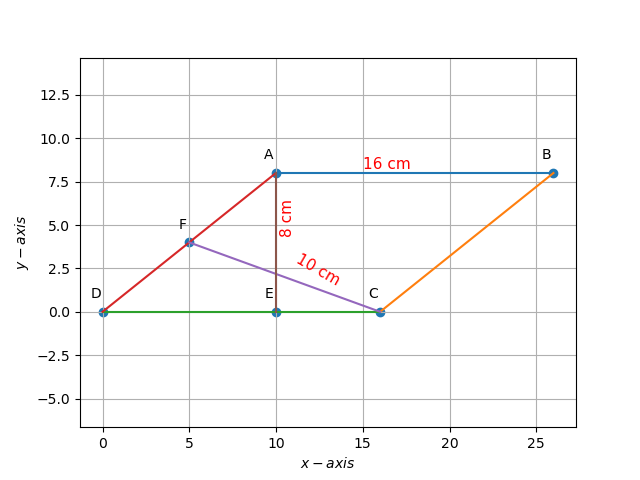
\includegraphics[width=\columnwidth]{fig1.png}
 \end{center}
 \caption{Parallelogram ABCD}
 \label{fig:Fig}
\end{figure}\\
\pagebreak
The following table consists of given input parameters of the above parallelogram ABCD :\\
\begin{table}[h]
\centering
	\begin{tabular}{|c|c|c|}
\hline
Symbol & Value & Description\\
\hline
$x$ & 16cm & $\vec{AB}$ \\
\hline
$a$ & 10cm & $\vec{CF}$ \\
\hline
$b$ & 8cm & $\vec{AE}$ \\
\hline
$\angle{CFD}$ & $90\degree$ & $CF \perp AD$ \\
\hline
$\angle{AED}$ & $90\degree$ & $AE \perp CD$ \\
\hline
\end{tabular}

	\caption{Parameters}
	\label{tab:table1}
\end{table}\\
Table below has the given input co-ordinates of the parallelogram :\\
\begin{table}[h]
	\centering
	\begin{tabular}{|p{2cm}|p{2cm}|p{2cm}|}
\hline
\multicolumn{3}{|c|}{Truth table}\\
\hline
R& S& A\\
\hline
0& 0& 0\\
\hline
0& 1& 1\\
\hline
1& 0& 1\\
\hline
1& 1& 0\\
\hline
\end{tabular}

	\caption{Co-ordinates}
	\label{tab:table2}
\end{table}\\
Following table shows the symbols and it's corresponding descriptions :\\
\begin{table}[h]
	\centering
	\begin{tabular}{|c|c|c|}
\hline
Symbol & Description\\
\hline
c & $\norm{\vec{D} -\vec{C}}$ \\
\hline
r & $\norm{\vec{A} -\vec{D}}$ \\
\hline
d & $\norm{\vec{D} - \vec{E}}$\\
\hline
b & $\norm{\vec{A} - \vec{E}}$\\
\hline
$\theta$ & $\angle{\vec{D}}$ \\
\hline
\end{tabular}

	\caption{Symbols and Corresponding Vectors}
	\label{tab:table3}
\end{table}\\
Rest of the point co-ordinates are derived in the following way : \\
\begin{align}
	\vec{C} = ce_1,\vec{A} = r\myvec{\cos{\theta}\\\sin{\theta}},\vec{B} = \vec{A} + \vec{C},\vec{E} = de_1,\vec{F} = \frac{k\vec{A} + \vec{D}}{k + 1}
\end{align}
\begin{enumerate}
	\item \textbf{To derive the co-ordinates of C :}\\
		As mentioned in the table3, $\norm{\vec{D} - \vec{C}} = c$.In the above parallelogram it is given that $\norm{\vec{B} - \vec{A}} = 16cm$.According to the properties of a parallelogram the parallel sides are equal in length.So, it can be said that : \\
		\begin{align}
			\norm{\vec{B} - \vec{A}} = \norm{\vec{D} - \vec{C}} = 16 = c\\
		\end{align}
As point $\vec{C}$ lies on x axis, it can be expressed in the following way :\\
		\begin{align}
			\vec{C} = ce_1\\
			\implies (16)\myvec{1\\0}\\
			\vec{C} = \myvec{16\\0}\\
		\end{align}
	\item \textbf{To derive the co-ordinates of A :}\\
		A can be expressed in the form of $r\myvec{\cos{\theta}\\\sin{\theta}}$.In order to obtain r and $\theta$, the following can be done : \\
		\begin{enumerate}
			\item \textbf{To find out $\theta$ :}\\
		To find out $\theta$,let us assume that $\norm{\vec{C} - \vec{F}} = a$		
		\begin{align}
			from \triangle{CFD},\\
			\sin{\theta} = \frac{a}{c}\\
			\implies \sin{\theta} = \frac{10}{16}\\
			\implies \sin^{-1}{\frac{10}{16}} = 38.68\degree\\
		\end{align}
	\item \textbf{To find out r :}\\
		As mentioned in table3, $\norm{\vec{D} - \vec{A}} = r$ and $\norm{\vec{E} - \vec{A}} = b$.In order to find out $r$,
		\begin{align}
			from \triangle{ADE},\\
			\sin{\theta} = \frac{b}{r}\\
			r = \frac{b}{\sin{\theta}}\\
			r = \frac{8}{\sin{\theta}}\\
			\implies \frac{8}{\frac{5}{8}}\\
			r = 12.8\\
		\end{align}
		So, the co-ordinates of $\vec{A}$ can be written as :\\
		\begin{align}
			\vec{A} = r\myvec{\cos{\theta}\\\sin{\theta}} = 12.8\myvec{\cos{38.68}\\\sin{38.68}}\\
			\implies \vec{A} = \myvec{10\\8} \\
		\end{align}
		\end{enumerate}
	\item \textbf{To find out the co-ordinates of B :}\\
		From parallelogram law of vectors, $\vec{B}$ can be expressed as the sum of $\vec{A}$ and $\vec{C}$.So, it can be written as,\\
		\begin{align}
			\vec{B} = \vec{A} + \vec{C}\\
			\vec{B} = \myvec{10\\8} + \myvec{16\\0}\\
			\vec{B} = \myvec{26\\8}\\
		\end{align}
	\item \textbf{To find out the co-ordinates of E :}\\
		As mentioned in the table3, $\norm{\vec{D} - \vec{E}} = d$.As, $\vec{E}$ lies on x-axis it can be written in the form of $de_1$.So, the co-ordinates can be found out in the following way : \\
		\begin{align}
			from \triangle{DAE},\\
			\cos{\theta} = \frac{d}{r}\\
			d = r\cos{\theta}\\
			\implies (12.8)\cos{38.68} \\
			\implies d = 10\\
		\end{align}
		 $\vec{E}$ = $de_1$ = (10)$\myvec{1\\0}$ = $\myvec{10\\0}$.\\
	 \item \textbf{To find out the co-ordinates of F :}\\
		 As point $\vec{F}$ divides $\vec{AD}$ in the ratio 39 : 1.The co-ordinates of $\vec{F}$ can be found out in the following way : \\
		 \begin{align}
			 \vec{F} = \frac{k\vec{A} + \vec{D}}{k + 1}\\
			 \vec{F} = \frac{(39)\myvec{10\\8} + \myvec{0\\0}}{40}\\
			 \vec{F} = \frac{1}{40}\myvec{390\\312}\\
			 \vec{F} = \myvec{9.75\\7.8}\\
		 \end{align}
\end{enumerate}
		 The length of $\vec{D} - \vec{A}$ was found out in the above process and it is $\norm{\vec{AD}} = \vec{r} = 12.8cm$.
\end{document}
